% Created by tikzDevice version 0.12.6 on 2026-08-03 04:29:06
% !TEX encoding = UTF-8 Unicode
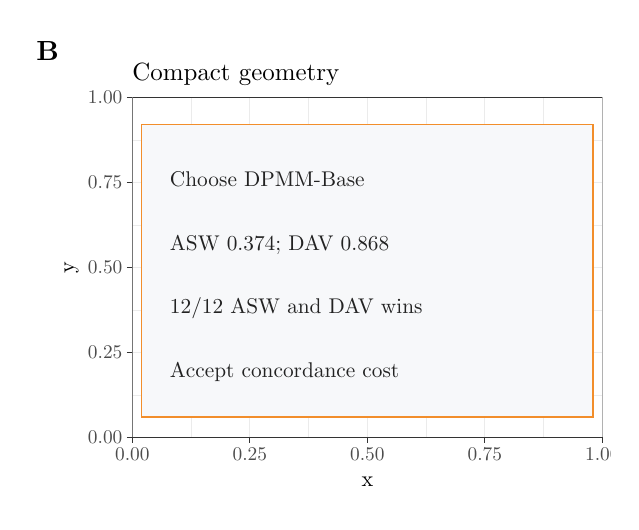
\begin{tikzpicture}[x=1pt,y=1pt]
\definecolor{fillColor}{RGB}{255,255,255}
\path[use as bounding box,fill=fillColor,fill opacity=0.00] (0,0) rectangle (210.78,171.36);
\begin{scope}
\path[clip] (  1.11,  1.87) rectangle (209.67,169.49);
\definecolor{drawColor}{RGB}{255,255,255}
\definecolor{fillColor}{RGB}{255,255,255}

\path[draw=drawColor,line width= 0.4pt,line join=round,line cap=round,fill=fillColor] (  1.11,  1.87) rectangle (209.67,169.49);
\end{scope}
\begin{scope}
\path[clip] ( 37.84, 23.34) rectangle (207.67,146.20);
\definecolor{fillColor}{RGB}{255,255,255}

\path[fill=fillColor] ( 37.84, 23.34) rectangle (207.67,146.20);
\definecolor{drawColor}{gray}{0.92}

\path[draw=drawColor,line width= 0.2pt,line join=round] ( 37.84, 38.69) --
	(207.67, 38.69);

\path[draw=drawColor,line width= 0.2pt,line join=round] ( 37.84, 69.41) --
	(207.67, 69.41);

\path[draw=drawColor,line width= 0.2pt,line join=round] ( 37.84,100.12) --
	(207.67,100.12);

\path[draw=drawColor,line width= 0.2pt,line join=round] ( 37.84,130.84) --
	(207.67,130.84);

\path[draw=drawColor,line width= 0.2pt,line join=round] ( 59.06, 23.34) --
	( 59.06,146.20);

\path[draw=drawColor,line width= 0.2pt,line join=round] (101.52, 23.34) --
	(101.52,146.20);

\path[draw=drawColor,line width= 0.2pt,line join=round] (143.98, 23.34) --
	(143.98,146.20);

\path[draw=drawColor,line width= 0.2pt,line join=round] (186.44, 23.34) --
	(186.44,146.20);

\path[draw=drawColor,line width= 0.4pt,line join=round] ( 37.84, 23.34) --
	(207.67, 23.34);

\path[draw=drawColor,line width= 0.4pt,line join=round] ( 37.84, 54.05) --
	(207.67, 54.05);

\path[draw=drawColor,line width= 0.4pt,line join=round] ( 37.84, 84.77) --
	(207.67, 84.77);

\path[draw=drawColor,line width= 0.4pt,line join=round] ( 37.84,115.48) --
	(207.67,115.48);

\path[draw=drawColor,line width= 0.4pt,line join=round] ( 37.84,146.20) --
	(207.67,146.20);

\path[draw=drawColor,line width= 0.4pt,line join=round] ( 37.84, 23.34) --
	( 37.84,146.20);

\path[draw=drawColor,line width= 0.4pt,line join=round] ( 80.29, 23.34) --
	( 80.29,146.20);

\path[draw=drawColor,line width= 0.4pt,line join=round] (122.75, 23.34) --
	(122.75,146.20);

\path[draw=drawColor,line width= 0.4pt,line join=round] (165.21, 23.34) --
	(165.21,146.20);

\path[draw=drawColor,line width= 0.4pt,line join=round] (207.67, 23.34) --
	(207.67,146.20);
\definecolor{drawColor}{RGB}{242,142,43}
\definecolor{fillColor}{RGB}{247,248,250}

\path[draw=drawColor,line width= 0.5pt,fill=fillColor] ( 41.23, 30.71) rectangle (204.27,136.37);
\definecolor{drawColor}{RGB}{34,34,34}

\node[text=drawColor,anchor=base west,inner sep=0pt, outer sep=0pt, scale=  0.77] at ( 51.42,113.88) {Choose DPMM-Base};

\node[text=drawColor,anchor=base west,inner sep=0pt, outer sep=0pt, scale=  0.77] at ( 51.42, 90.94) {ASW 0.374; DAV 0.868};

\node[text=drawColor,anchor=base west,inner sep=0pt, outer sep=0pt, scale=  0.77] at ( 51.42, 68.01) {12/12 ASW and DAV wins};

\node[text=drawColor,anchor=base west,inner sep=0pt, outer sep=0pt, scale=  0.77] at ( 51.42, 45.08) {Accept concordance cost};
\definecolor{drawColor}{gray}{0.20}

\path[draw=drawColor,line width= 0.4pt,line join=round,line cap=round] ( 37.84, 23.34) rectangle (207.67,146.20);
\end{scope}
\begin{scope}
\path[clip] (  0.00,  0.00) rectangle (210.78,171.36);
\definecolor{drawColor}{gray}{0.30}

\node[text=drawColor,anchor=base east,inner sep=0pt, outer sep=0pt, scale=  0.70] at ( 34.24, 20.93) {0.00};

\node[text=drawColor,anchor=base east,inner sep=0pt, outer sep=0pt, scale=  0.70] at ( 34.24, 51.64) {0.25};

\node[text=drawColor,anchor=base east,inner sep=0pt, outer sep=0pt, scale=  0.70] at ( 34.24, 82.36) {0.50};

\node[text=drawColor,anchor=base east,inner sep=0pt, outer sep=0pt, scale=  0.70] at ( 34.24,113.07) {0.75};

\node[text=drawColor,anchor=base east,inner sep=0pt, outer sep=0pt, scale=  0.70] at ( 34.24,143.79) {1.00};
\end{scope}
\begin{scope}
\path[clip] (  0.00,  0.00) rectangle (210.78,171.36);
\definecolor{drawColor}{gray}{0.20}

\path[draw=drawColor,line width= 0.4pt,line join=round] ( 35.84, 23.34) --
	( 37.84, 23.34);

\path[draw=drawColor,line width= 0.4pt,line join=round] ( 35.84, 54.05) --
	( 37.84, 54.05);

\path[draw=drawColor,line width= 0.4pt,line join=round] ( 35.84, 84.77) --
	( 37.84, 84.77);

\path[draw=drawColor,line width= 0.4pt,line join=round] ( 35.84,115.48) --
	( 37.84,115.48);

\path[draw=drawColor,line width= 0.4pt,line join=round] ( 35.84,146.20) --
	( 37.84,146.20);
\end{scope}
\begin{scope}
\path[clip] (  0.00,  0.00) rectangle (210.78,171.36);
\definecolor{drawColor}{gray}{0.20}

\path[draw=drawColor,line width= 0.4pt,line join=round] ( 37.84, 21.34) --
	( 37.84, 23.34);

\path[draw=drawColor,line width= 0.4pt,line join=round] ( 80.29, 21.34) --
	( 80.29, 23.34);

\path[draw=drawColor,line width= 0.4pt,line join=round] (122.75, 21.34) --
	(122.75, 23.34);

\path[draw=drawColor,line width= 0.4pt,line join=round] (165.21, 21.34) --
	(165.21, 23.34);

\path[draw=drawColor,line width= 0.4pt,line join=round] (207.67, 21.34) --
	(207.67, 23.34);
\end{scope}
\begin{scope}
\path[clip] (  0.00,  0.00) rectangle (210.78,171.36);
\definecolor{drawColor}{gray}{0.30}

\node[text=drawColor,anchor=base,inner sep=0pt, outer sep=0pt, scale=  0.70] at ( 37.84, 14.92) {0.00};

\node[text=drawColor,anchor=base,inner sep=0pt, outer sep=0pt, scale=  0.70] at ( 80.29, 14.92) {0.25};

\node[text=drawColor,anchor=base,inner sep=0pt, outer sep=0pt, scale=  0.70] at (122.75, 14.92) {0.50};

\node[text=drawColor,anchor=base,inner sep=0pt, outer sep=0pt, scale=  0.70] at (165.21, 14.92) {0.75};

\node[text=drawColor,anchor=base,inner sep=0pt, outer sep=0pt, scale=  0.70] at (207.67, 14.92) {1.00};
\end{scope}
\begin{scope}
\path[clip] (  0.00,  0.00) rectangle (210.78,171.36);
\definecolor{drawColor}{RGB}{0,0,0}

\node[text=drawColor,anchor=base,inner sep=0pt, outer sep=0pt, scale=  0.80] at (122.75,  5.64) {x};
\end{scope}
\begin{scope}
\path[clip] (  0.00,  0.00) rectangle (210.78,171.36);
\definecolor{drawColor}{RGB}{0,0,0}

\node[text=drawColor,rotate= 90.00,anchor=base,inner sep=0pt, outer sep=0pt, scale=  0.80] at ( 16.80, 84.77) {y};
\end{scope}
\begin{scope}
\path[clip] (  0.00,  0.00) rectangle (210.78,171.36);
\definecolor{drawColor}{RGB}{0,0,0}

\node[text=drawColor,anchor=base west,inner sep=0pt, outer sep=0pt, scale=  0.90] at ( 37.84,152.18) {Compact geometry};
\end{scope}
\begin{scope}
\path[clip] (  0.00,  0.00) rectangle (210.78,171.36);
\definecolor{drawColor}{RGB}{0,0,0}

\node[text=drawColor,anchor=base,inner sep=0pt, outer sep=0pt, scale=  1.00] at (  7.20,159.49) {\bfseries B};
\end{scope}
\end{tikzpicture}
